\documentclass[12pt]{article}
\usepackage{lipsum}   % for filler text
\usepackage{setspace} % for \onehalfspacing and \singlespacing macros
\onehalfspacing 
\usepackage{blindtext}
\usepackage[english]{babel}
\usepackage{biblatex}
\usepackage{csquotes}
\usepackage{xargs}                      % Use more than one optional parameter in a new commands
\usepackage[pdftex,dvipsnames]{xcolor}  % Coloured text etc.
\usepackage{mathtools}
\usepackage{amssymb}
\usepackage[a4paper, total={6in, 8in}]{geometry}
\newcommand{\argmax}{\operatornamewithlimits{argmax}}

% 
\usepackage[colorinlistoftodos,prependcaption,textsize=tiny]{todonotes}
\newcommandx{\unsure}[2][1=]{\todo[linecolor=red,backgroundcolor=red!25,bordercolor=red,#1]{#2}}
\newcommandx{\change}[2][1=]{\todo[linecolor=blue,backgroundcolor=blue!25,bordercolor=blue,#1]{#2}}
\newcommandx{\info}[2][1=]{\todo[linecolor=OliveGreen,backgroundcolor=OliveGreen!25,bordercolor=OliveGreen,#1]{#2}}
\newcommandx{\improvement}[2][1=]{\todo[linecolor=Plum,backgroundcolor=Plum!25,bordercolor=Plum,#1]{#2}}
\newcommandx{\thiswillnotshow}[2][1=]{\todo[disable,#1]{#2}}
%

\addbibresource{biblo.bib}
\graphicspath{ {images/} }

\title{COMP 551: Applied Machine Learning Notes}
\date{2020\\ September}
\author{Brendan Kellam}
\begin{document}
\maketitle
\section{Preamble}
This document will act as a running set of notes for COMP 551, Applied Machine Learning \cite{551website}. My objective with this document is to provide a summarized version of the course.

\section{Introduction to Machine Learning}
What exactly \textbf{is} "machine learning"? I like Kevin P. Murphy's definition from his book "Machine Learning: A Probabilistic Perspective": 

\begin{quote}
"In particular, we define machine learning as a set of methods that can automatically detect patterns in data, and then use the uncovered patterns to predict future data, or to perform other kinds of decision making under uncertainty (such as planning how to collect more data!)" \cite{murphy}
\end{quote}

To solve such problems, we can utilize the tools of probability theory. \improvement{A summarized review of probability theory would be useful.}

\section{Types of machine learning}
In the following section, we will review the main "types" of machine learning and go over a brief introduction into the different variations for each.

\subsection{Supervised / predictive learning}
Goal: learn a mapping from inputs \(\mathbf{x}\) to outputs \(y\)
\newline
Given:
\[
    \mathcal{D} = \lbrace (\mathbf{x}_i, y_i) \rbrace_{i=1}^{N}.
\]
\newline
Where:
\begin{itemize}
    \item \(\mathcal{D} - \text{training set}\)
    \item \(N - \text{number of training examples}\)
    \item \(\mathbf{x}_i - \text{input (e.g. a D-dimensional vector)}\). Each element \(\in \mathbf{x}\) is known as a \textbf{feature/attribute/covariant}. \(\mathbf{x}_i\) could be a complex structured object, like a image, sentence, etc.
    \item \(y_i - \text{output/response variable.}\) \(y_i\) is typically either a \textbf{categorical/nominal} variable from a finite set \(y_i \in \lbrace 1,\dots,C\rbrace\) (e.g. \(y_i \in \lbrace male, female \rbrace\)) \textbf{or} a \textbf{real-valued scalar} \(y_i \in \mathbb{R}\) (e.g. income level).
\end{itemize}
\bigskip
\textbf{Note:} If \(y_i\) is categorical \(\implies\) the problem is known as \textbf{classification/pattern recognition}. Otherwise, if \(y_i\) is real-valued \(\implies\) the problem is \textbf{regression}.


\subsubsection{Classification}
We can formalize the problem of classification by viewing it via the lense of \textbf{function approximation} \cite{murphy}. We assume \(y = f(\mathbf{x})\) for some unknown function \(f\). The goal of \textbf{learning} is to estimate this function \(f\) given a labeled training set, and then to make predictions using \(\hat{y} = \hat{f}(\mathbf{x})\) (Where the hat denotes a estimate.) We can then use our estimate \(\hat{f}\) to make predictions on inputs that do not exist within our training set (i.e. some \(\mathbf{x}\) s.t. \(\mathbf{x} \notin \mathcal{D}\)).
\newline
\textbf{Example:}
\newline
Figure \ref{fig:classificationex1} depicts a simple classification example where we are tying to classify objects with three features (\( \lbrace \text{color, shape, size} \rbrace \in \mathbf{x_i} \)) into two catagories (\(\lbrace \text{yes, no} \rbrace \in y_i\)).
\begin{figure}[h]
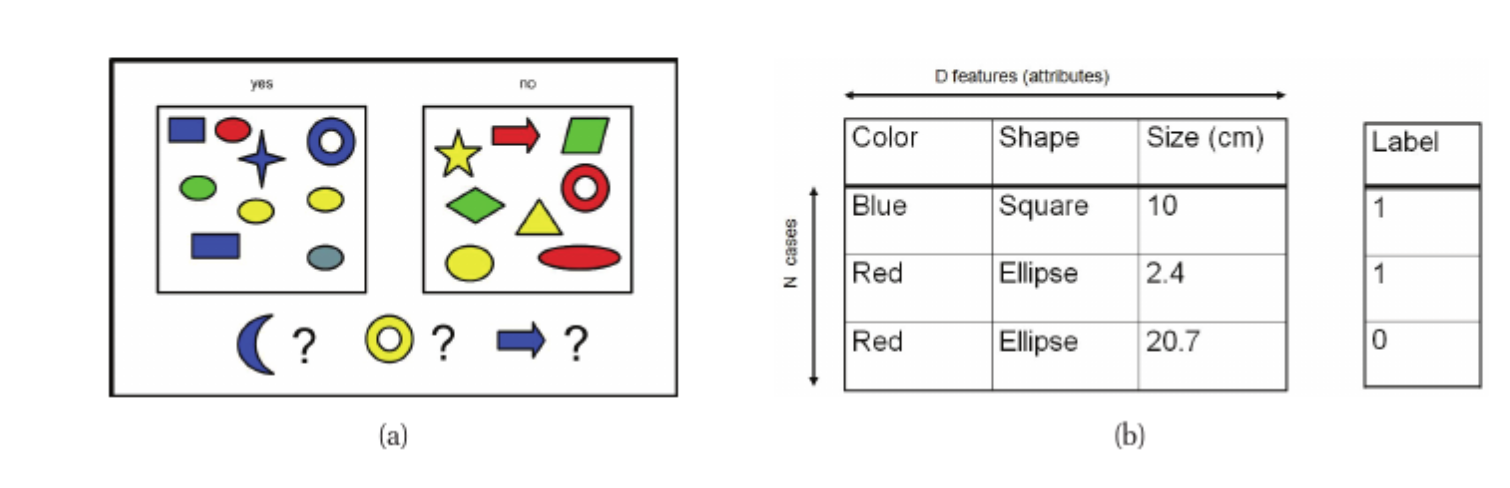
\includegraphics[width=\textwidth]{murphy-fig-1-1.png}
\caption{(a) Labeled training examples along with 3 unlabeled test cases. (b) \(N x D\) design matrix representing our training data. Each row is a feature vector \(\mathbf{x}_i\). Last column is the label, \(y_i \in \lbrace 0, 1 \rbrace \) \cite{murphy}}
\label{fig:classificationex1}
\end{figure}

In the example, predicting the label for the moon is quite clear (it will likely be assigned a "yes" label since all training examples with color blue exist within this category). A classification for the yellow circle is less certain: there are training examples with color yellow and shape circle in both catagories. This notion of ambiguity in our estimations motivates the need for a probability metric. 

The probability distribution over possible labels, given input vector \(\mathbf{x}\) and training set \(\mathcal{D}\), is given by \(p(y|\textbf{x},\mathcal{D}) \). This represents a vector of length \(C\) (e.g. given \(\mathbf{x}_i = \text{[Blue, Square, 10]}\), we may expect \(p(y|\mathbf{x}_i,\mathcal{D}) \) = [0.2, 0.8], implying we are 80\% sure \(\mathbf{x}_i\) should be labeled as 1). We can compute our "best guess" as to the "true label" by using:
\begin{equation}
\hat{y} = \hat{f}(\mathbf{x}) = \argmax_{c=1}^C p(y = c|\mathbf{x},\mathcal{D})
\label{eq:MAPEstimate}
\end{equation}
(\ref{eq:MAPEstimate}) corresponds to the most probable class label and is also known as the \textbf{MAP} estimate (Maximum A Posteriori). In the case of the yellow circle from Figure \ref{fig:classificationex1}, we could expect \(p(\hat{y}|\mathbf{x},\mathcal{D})\) being far from 1.0 (i.e. we are not confident of our classification).

\textbf{NOTE:} we are implicitly conditioning our classification probabilities on the chosen model. When needed, we can explicitly denote a conditional on a model by writing \(p(y|\textbf{x},\mathcal{D}, M)\) where \(M\) is our chosen model. 

\subsubsection{Regression}
TODO

\subsection{Unsupervised / descriptive learning}
Goal: learn a mapping from inputs \(\mathbf{x}\) to outputs \(y\)
\newline
Given:
\[
    \mathcal{D} = \lbrace \mathbf{x}_i \rbrace_{i=1}^{N}.
\]

\subsection{Reinforcement learning}
Goal: Learn how to act/behave when given occasional reward or punishment signals.

\section{KNN}
TODO

\printbibliography


\end{document}